%!TEX root = main.tex

\lectureheader{161}{Calculus I}{Trigonometry review}{\textit{Thomas' Calculus} 1.3}

\begin{theorem}
The circumference of a circle of radius $r$ is $C=2\pi r$.
\end{theorem}

\begin{definition}
The \textbf{radian measure} of a counterclockwise-oriented, central angle within a circle of radius $r$ is $$\theta = s/r,$$ where $s$ is the length of the arc subtended by the angle.
\end{definition}

\begin{figure}[H]
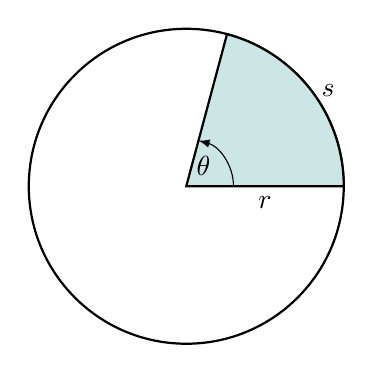
\begin{tikzpicture}[scale=2]
\draw[thick] (0,0) circle (1cm);
\filldraw[thick, fill=teal!20!]
(0,0) node[above right]{$\theta$} -- (1cm,0mm) node[midway, below]{$r$}  arc (0:75:1cm) node[midway, right]{$s$} -- cycle;
\draw[-latex] (0.3cm,0) arc(0:75:0.3cm) node[midway, below]{};
\end{tikzpicture}
\end{figure}

\begin{remark}\,
\begin{itemize}
\item As the ratio of 2 lengths (measured according to the same unit of length), radians are \textbf{unitless}.
\item Clockwise orientation is indicated by negative measure.
\item There are exactly $2\pi$ radians in one full turn of a circle.
\item In calculus, we alway default to radian measure (e.g., $\theta=60$ means 60 radians, not 60\textdegree).
\item $1^\circ=\frac{\pi}{180}$
\end{itemize}
\end{remark}

\newpage

\begin{definition}
Given an angle in standard position (vertex at the origin, initial side along the positive $x$-axis), of measure $\theta$ (radians), and a point $P(x,y)$ on the terminal side at distance $r$ from the origin, 
we define the 6 basic trigonometric functions by
\begin{alignat*}{3}
&\sin\theta = \frac{y}{r},\quad && \cos\theta = \frac{x}{r},\quad && \tan\theta = \frac{y}{x},\\
\\
&\csc\theta = \frac{1}{\sin\theta},\quad && \sec\theta = \frac{1}{\cos\theta},\quad && \cot\theta = \frac{1}{\tan\theta}.
\end{alignat*}
\end{definition}

\begin{figure}[H]
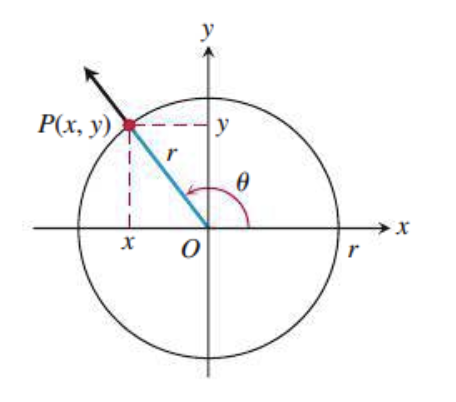
\includegraphics[width=3in]{img/trig_function_def}
\end{figure}

\begin{example}
Given that $\sin\theta = -3/5$ and $\theta\in [-\pi/2, 0]$,
find the values of the remaining trigonometric functions at $\theta$.
\end{example}


\newpage

\begin{figure}[H]\caption{Reference triangles}
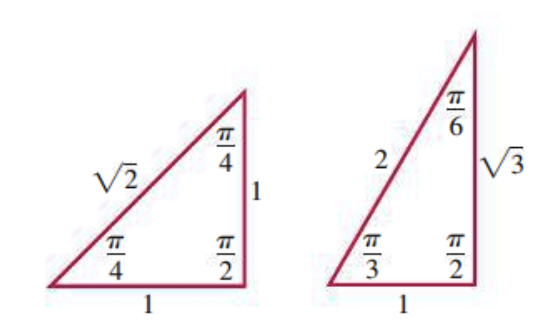
\includegraphics[width=3in]{img/ref_angles}
\end{figure}

\begin{example}
Evaluate all 6 trigonometric functions at $\theta = 2\pi/3$, $\theta=-5\pi/6$, and at $\theta=9\pi/4$.
\end{example}

\newpage

\begin{figure}[H]
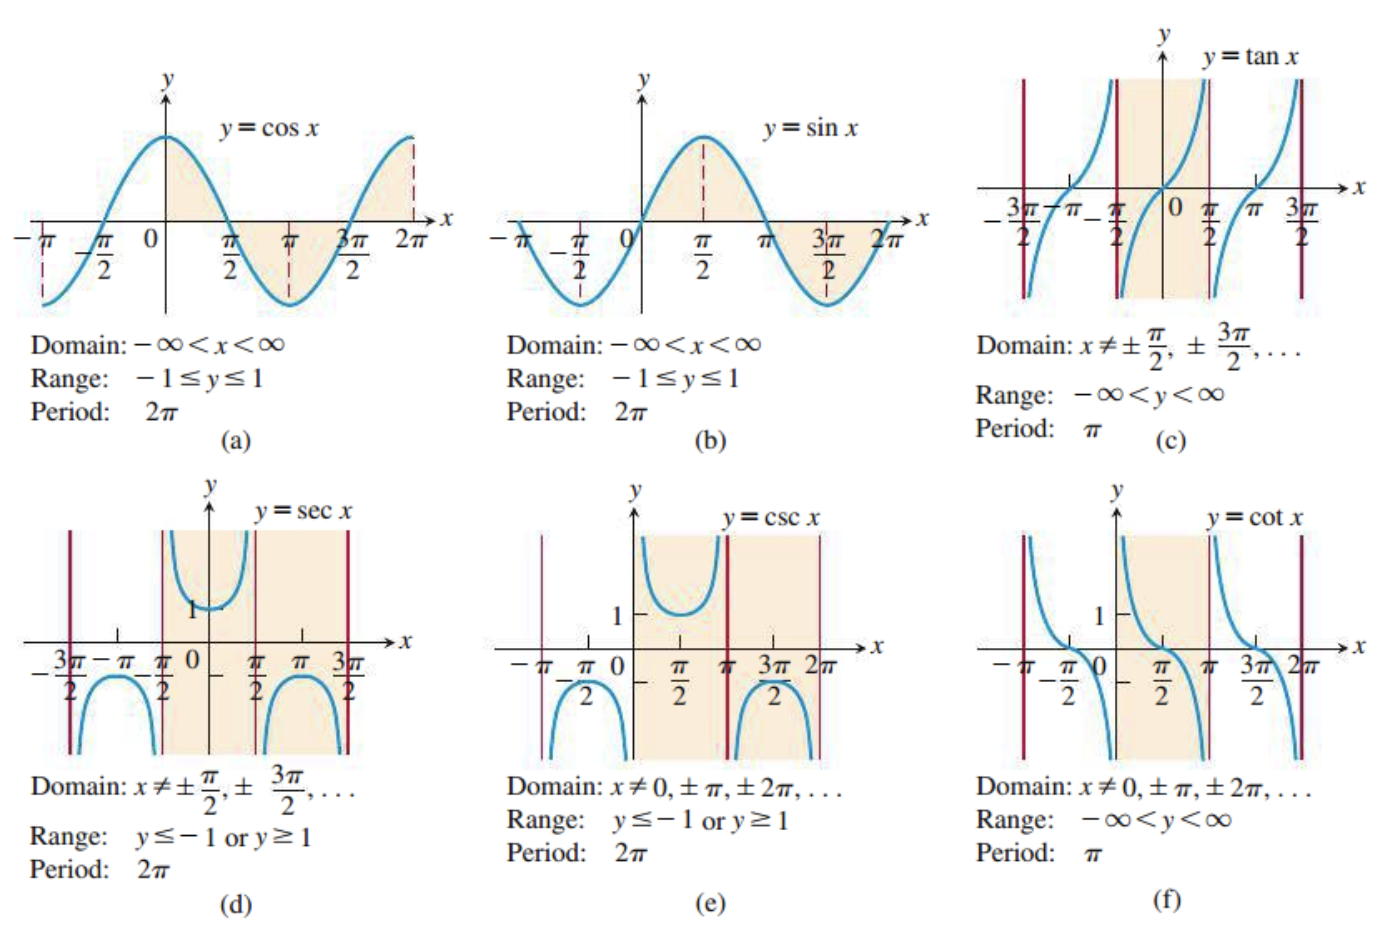
\includegraphics[width=7in]{img/trig_plots}
\end{figure}

\begin{definition}
A function $f$ is said to be \textbf{periodic} if there is a positive number $p$ so that
\begin{equation*}
f(x+p) = f(x)
\end{equation*}
for all $x\in\R$.
The smallest such value of $p$ is called the \textbf{period} of $f$.
\end{definition}

\begin{example}
Determine the period of $f(x)=2\sin(7x-1)+5$ and sketch its graph.
\end{example}


\newpage

\begin{theorem}[Pythagorean identities]
For all $\theta\in\R$,
\begin{align*}
\sin^2\theta + \cos^2\theta &= 1,\\
1+\tan^2\theta &= \sec^2\theta,\\
\cot^2\theta+1 &=\csc^2\theta.
\end{align*}
\end{theorem}
\vfill

\begin{theorem}[Addition identities]
For all $A,B\in\R$,
\begin{align*}
\cos(A+B) &=\cos A\cos B - \sin A\sin B,\\
\sin(A+B) &=\sin A\cos B+\cos A\sin B.
\end{align*}
\end{theorem}
\vfill

\begin{theorem}[Double-angle identities]
For all $\theta\in\R$,
\begin{align*}
\cos(2\theta) &= \cos^2\theta-\sin^2\theta,\\
\sin(2\theta) &= 2\sin\theta\cos\theta.
\end{align*}
\end{theorem}
\vfill

\begin{theorem}[Half-angle identities]
For all $\theta\in\R$,
\begin{align*}
\cos^2\theta &= \frac{1+\cos(2\theta)}{2},\\
\sin^2\theta &= \frac{1-\cos(2\theta)}{2}.
\end{align*}
\end{theorem}
\vfill

\begin{theorem}[Law of cosines]
If $a$, $b$, and $c$ are the side lengths of a triangle and $\theta$ is the measure of the angle opposite $c$, then
\begin{equation*}
c^2=a^2+b^2-2ab\cos\theta.
\end{equation*}
\end{theorem}
\vfill

\newpage

\begin{theorem}
For any $\theta\in\R$,
\begin{align*}
|\sin\theta|&\le |\theta|,\\
1-\cos\theta &\le |\theta|.
\end{align*}
\end{theorem}

